% General settings
\documentclass[slidestop,compress,9pt]{beamer}
\usetheme{AnnArbor}
\usepackage[UKenglish]{babel}
\usepackage[UKenglish]{isodate}
\usepackage[utf8]{inputenc}
\usepackage{hyperref}
\definecolor{links}{HTML}{2A1B81}
\hypersetup{colorlinks=true,allcolors=links}

% Code listings and pseudocode
\usepackage{listings}
\usepackage{algpseudocode}
\usepackage{algorithm}

% Mathematical formulas
\usepackage{amsmath}
\usepackage{mathtools}
\usepackage{bm}
\setcounter{MaxMatrixCols}{20}

% Graphics and figures
\usepackage{graphicx}
\graphicspath{{figures/}}
\setbeamertemplate{caption}[numbered]
\usepackage{fancybox}
\usepackage{pgfplots}

% Tikz
\usepackage{tikz}
\usepackage{tikz-3dplot}
\usetikzlibrary{shapes.geometric, arrows}

% For redefinition of texttt
%\let\textttorig\texttt
\usepackage[scaled=1.0]{couriers}

\setbeamertemplate{frametitle}{\thesection.~\insertsection\hspace*{0.45cm}\insertframetitle}

% Numbered sections
\setbeamertemplate{section in toc}[sections numbered]
\setbeamertemplate{subsection in toc}[subsections numbered]
\setbeamertemplate{subsubsection in toc}[subsubsections numbered]

% Listings
\definecolor{cident}{rgb}{0.0,0.0,0.0}
\definecolor{ckeyw}{rgb}{0,0,0.8}
\definecolor{ccomm}{rgb}{0,0.8,0}
\definecolor{cstr}{rgb}{0.8,0,0}
\definecolor{myyellow}{rgb}{0.99,0.76, 0.0}
\definecolor{mymagenta}{rgb}{1.0, 0.0, 1.0}

\lstset{language=[LaTeX]{TeX},
  basicstyle=\normalsize\ttfamily,
  keywordstyle=\color{ckeyw}\bfseries,
  identifierstyle=\color{cident}\bfseries,
  commentstyle=\color{ccomm},
  stringstyle=\color{cstr},
  showstringspaces=false,
  breaklines=true,
  breakatwhitespace=true,
  tabsize=2,
  mathescape = false,
  columns=flexible,
  escapeinside={<@}{@>}
%   numbers=left,
%   stepnumber=1,
%   firstnumber=1,
%   numberfirstline=true,
  }

\title[The oxDNA Coarse-Grained Model of DNA and RNA]{\textbf{The oxDNA Coarse-Grained Model of DNA}}
\subtitle{An Introduction to the Model and Software Framework }
\author[Oliver Henrich]{Oliver Henrich \\ \small Email: \href{mailto:oliver.henrich@strath.ac.uk}{oliver.henrich@strath.ac.uk}}
\institute[U Strathclyde, Glasgow, UK]{Department of Physics, University of Strathclyde, Glasgow, UK}
\date{22nd September 2022}


\begin{document}

%\renewcommand<>{\texttt}[1]{%
%  \only#2{\textttorig{#1}}%
%}

\renewcommand<>{\texttt}{\only#1{\beameroriginal{\texttt}}}

% ==============================================================
% --- Welcome frame
% ==============================================================
\begin{frame}[plain]
\maketitle
\end{frame}

% ==============================================================
% --- TOC
% ==============================================================

\begin{frame}
\Large Outline
\normalsize
\tableofcontents
\end{frame}

% ==============================================================
% --- Content
% ==============================================================

\section{oxDNA Model}

\begin{frame}
\frametitle{DNA Facts}

\begin{itemize}
\item Human genome contains $3\times10^{9}$ base pairs (bps)
\item DNA loop around a nucleosome core particle contains 147 bps
\item Smallest loop in chromatin fibre consists of $5\times10^4$ bps
\item Atomistic simulation of DNA can model 3,000 bps (probably less) and typically resolve times on the $\mu$s-scale  
\item Coarse-grained models target much larger time and length scales in the range of ms and Mbps 
\end{itemize}

\begin{center}
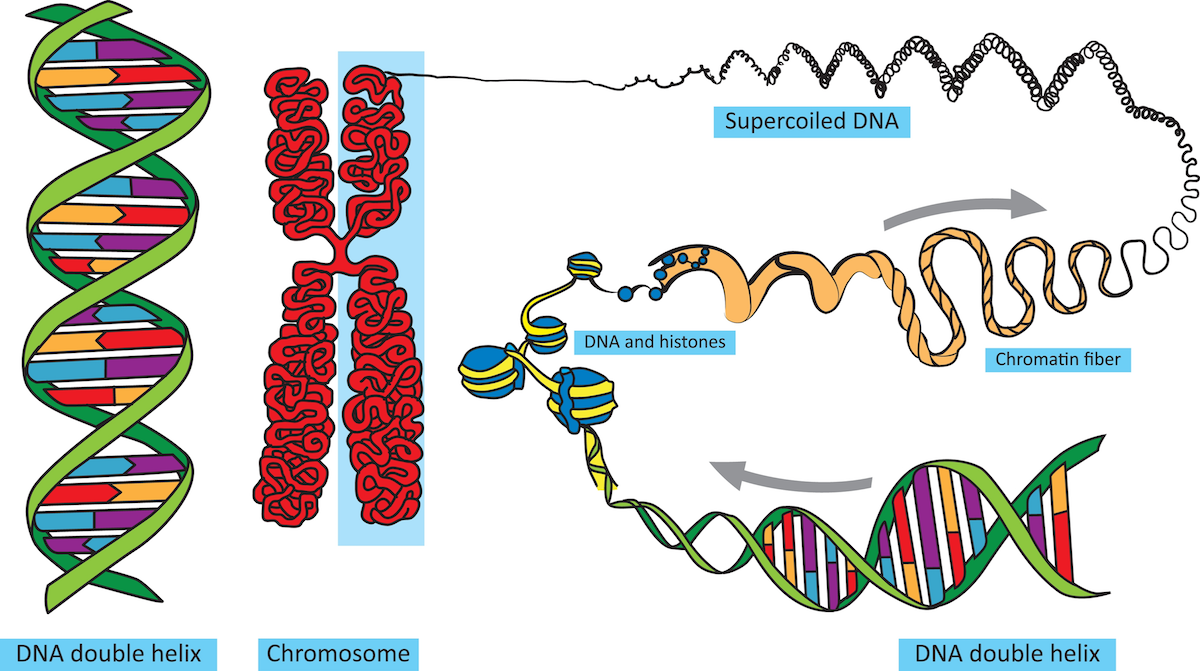
\includegraphics[width=0.54\textwidth]{fromDNAtoChromatin.png}
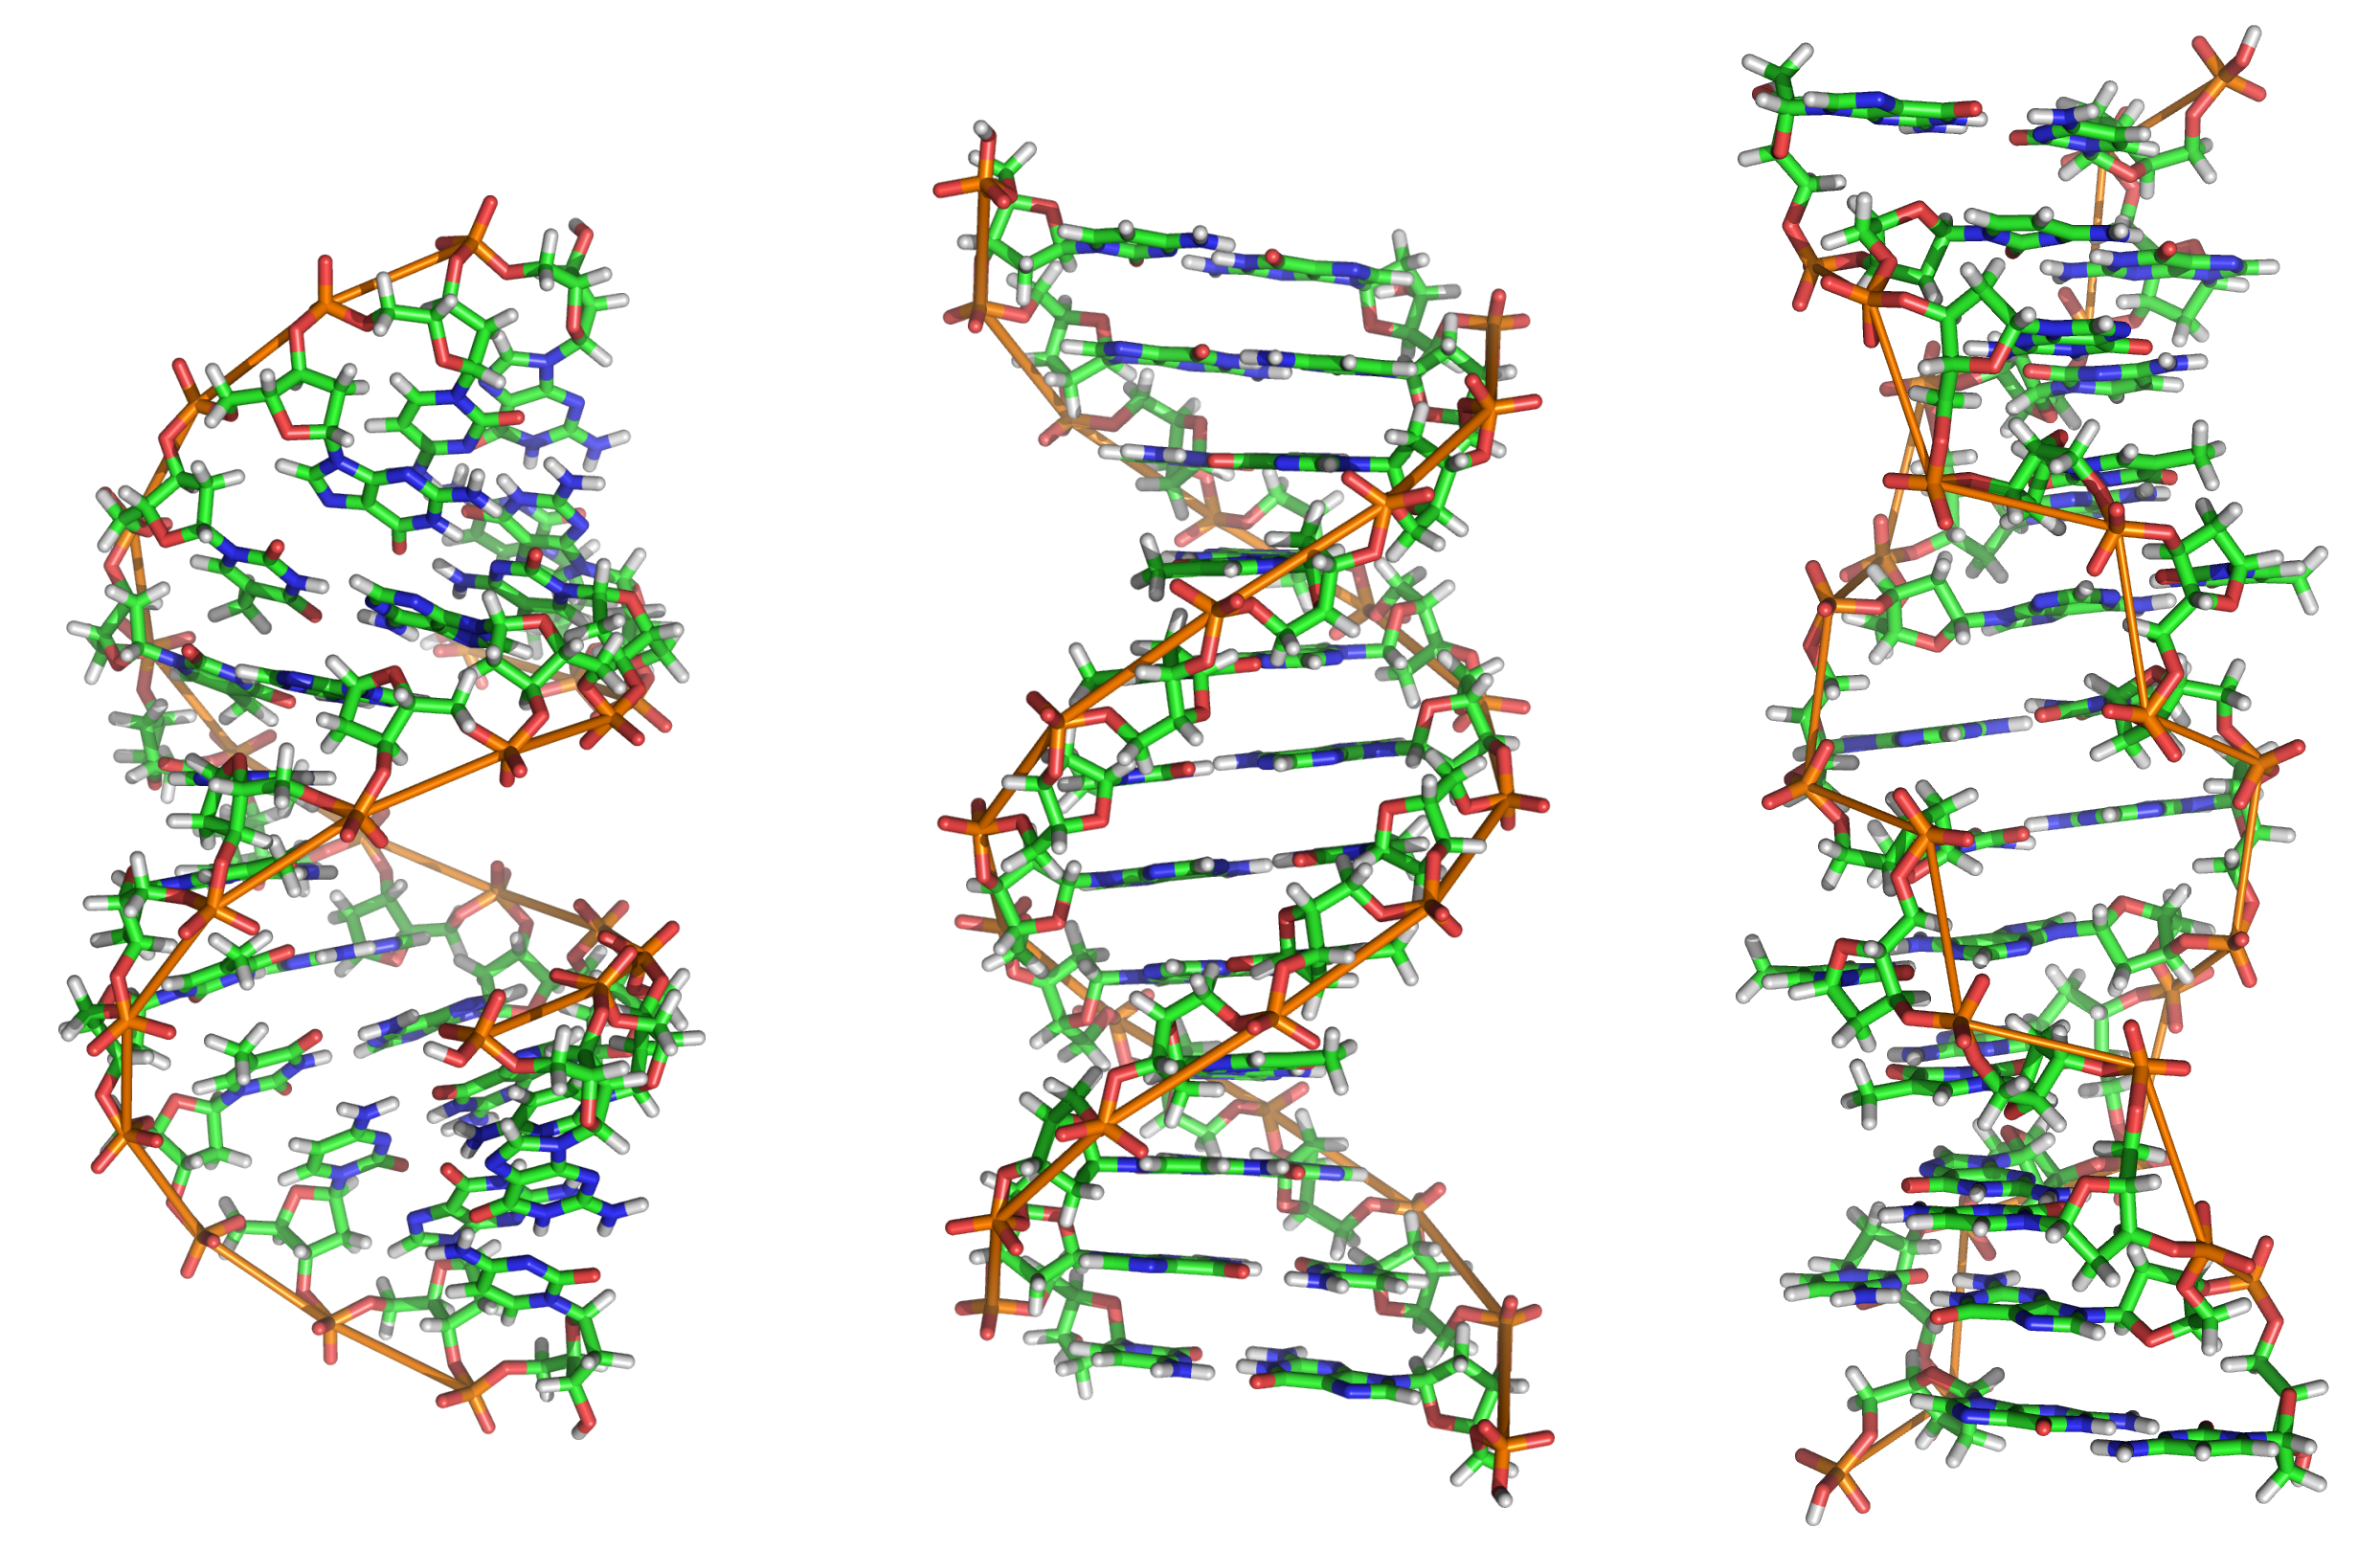
\includegraphics[width=0.45\textwidth]{A-B-Z-DNA.png}\\
From DNA to chromatin \hspace{2.75cm} A-DNA, B-DNA, Z-DNA
\end{center}

\end{frame}

\begin{frame}
\frametitle{Overview}

\begin{itemize}
\item Each nucleotide is described as rigid body
\item 3 interaction sites for backbone, stacking and hydrogen-bonding
\item 7 effective interactions between nucleotides
\begin{itemize}
\item Bonded interaction for backbone connectivity
\item 6 pair interactions for excluded volume, stacking, cross-stacking, coaxial stacking, hydrogen-bonding and electrostatic interaction
\end{itemize}
\item oxDNA: 13 DOF per nucleotide\\
3 positions, 3 translational momenta, 3 angular momenta, 1 unit quaternion (4 components)
\item Atomistic simulation (e.g. thymine): around 200 DOF per nucleotide\\
34 atoms per nucleotide, each with 3 positions and 3 momenta
\end{itemize}

\vspace*{-0.5cm}

\begin{columns}
\begin{column}{0.4\textwidth}
\begin{center}
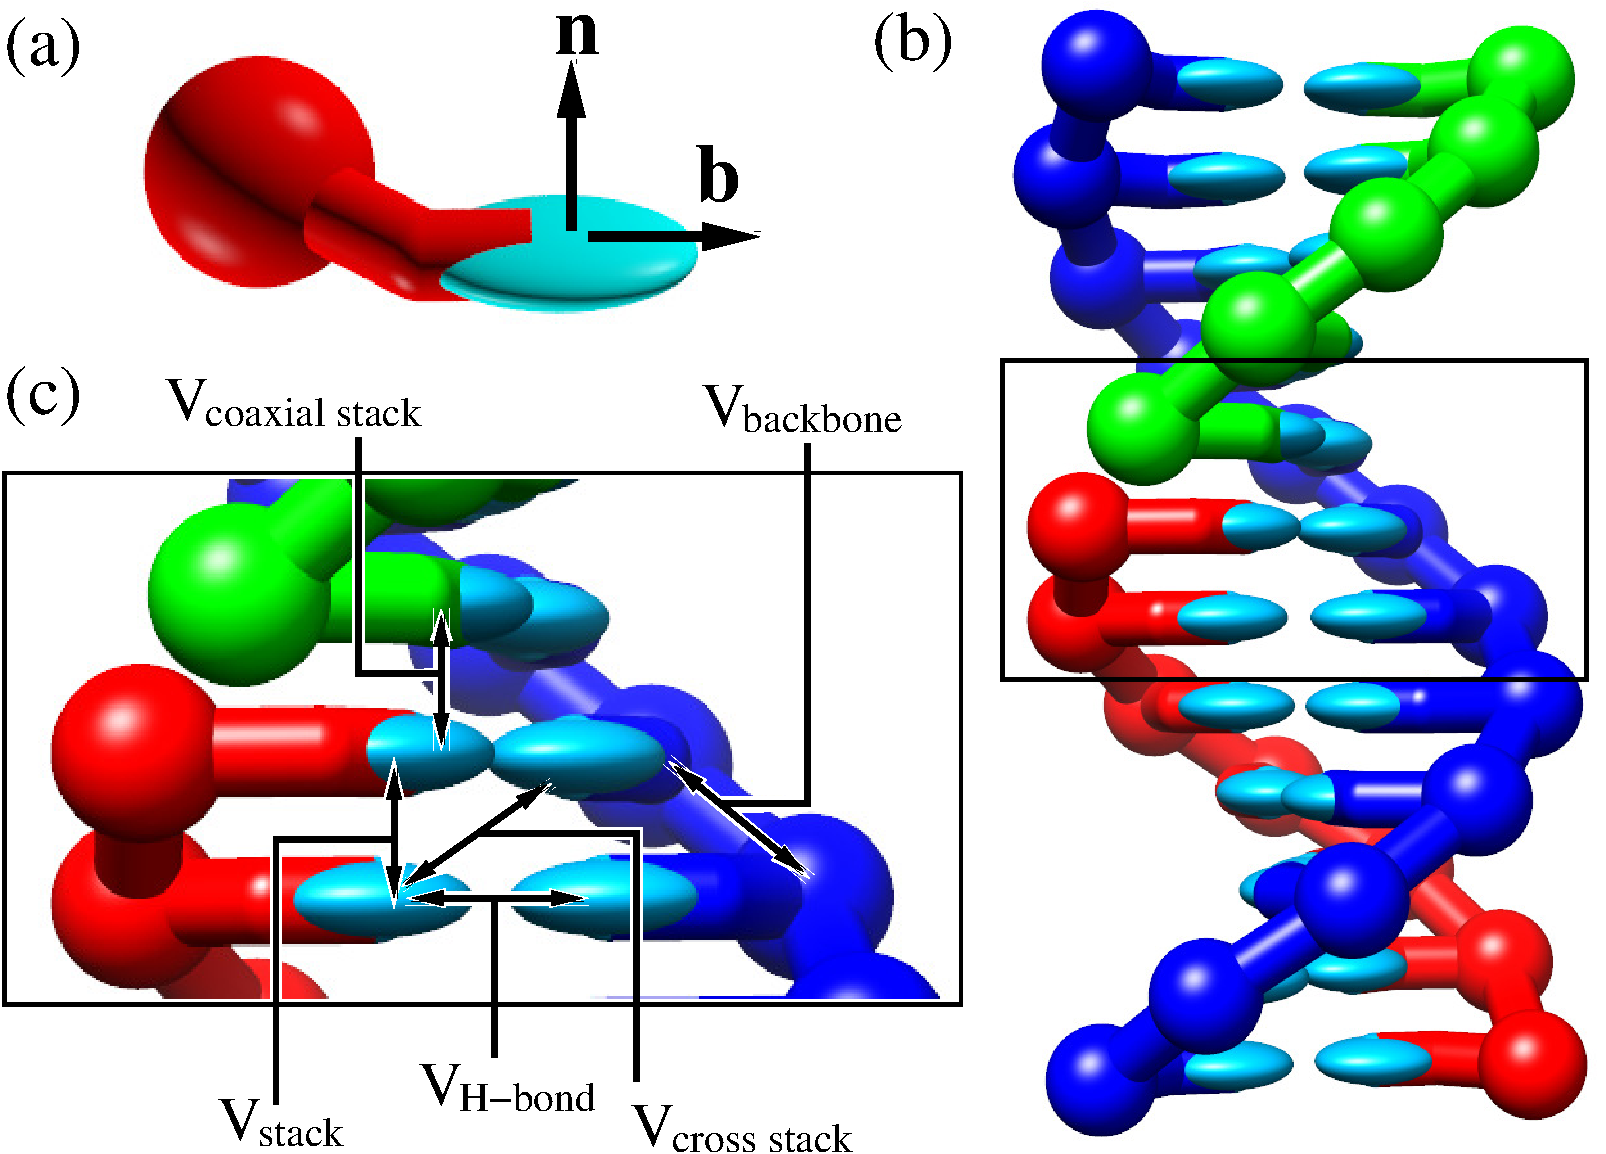
\includegraphics[width=0.9\textwidth]{nucleotide_duplex_b.pdf}
\end{center}
\end{column}

\begin{column}{0.45\textwidth}
\begin{center}
\vspace*{0.5cm}
\begin{itemize}
\setlength\itemsep{7pt}
\item[] (a) oxDNA nucleotide
\item[] (b) Duplex
\item[] (c) Interactions
\end{itemize}
\end{center}
\end{column}
\end{columns}

\end{frame}

\begin{frame}
\frametitle{Nucleotide Geometry}

\begin{columns}
\begin{column}{0.56\textwidth}
\begin{itemize}
\setlength\itemsep{20pt}
\item Each nucleotide has a centre of mass (COM) $\bm{r}_{COM}$, a base vector $\bm{b}$, base normal $\bm{n}$ and a third vector $\bm{y}=\bm{n}\times\bm{b}$
\item The \textbf{backbone interaction} site is at\\
$\bm{r}_{back}=\bm{r}_{COM} - 0.4\,\bm{b}$ \hspace{1.7cm}(oxDNA1)\\
$\bm{r}_{back}=\bm{r}_{COM} - 0.34\, \bm{b} + 0.3408\,\bm{y}$ (oxDNA2)
\item The \textbf{stacking interaction} site is at\\
$\bm{r}_{stack}=\bm{r}_{COM} + 0.34\, \bm{b}$
\item The \textbf{hydrogen-bonding interaction} site is at\\
$\bm{r}_{base}=\bm{r}_{COM} + 0.4\, \bm{b}$
\end{itemize}
\end{column}

\begin{column}{0.44\textwidth}
\vspace*{-0.5cm}
\begin{center}
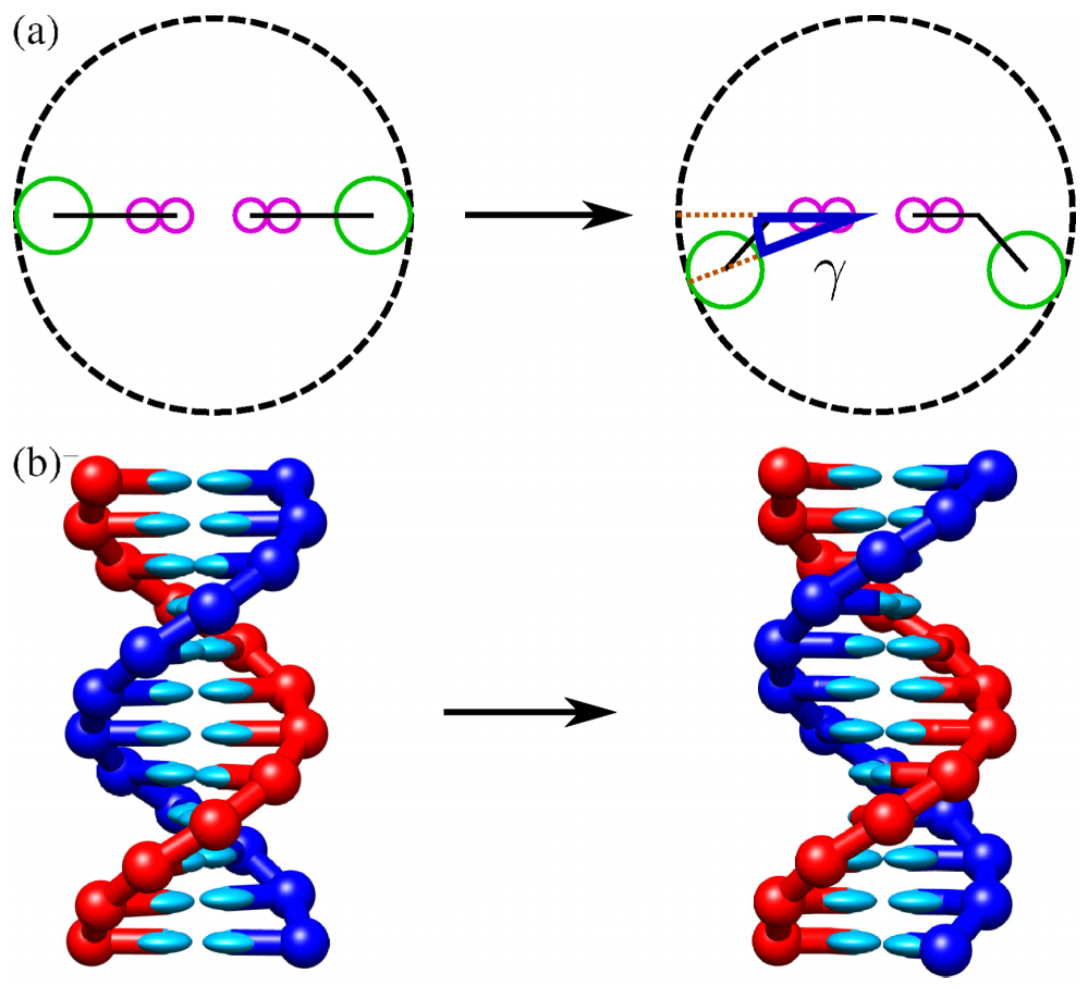
\includegraphics[width=0.85\textwidth]{oxdna_oxdna2.png}\\
\end{center}
(a) oxDNA1 and oxDNA2 nucleotides: the base vector $\bm{b}$ is horizontally oriented from left to right, whereas the base normal $\bm{n}$ points away from the observer.\\[3pt]
(b) The angled backbone interaction sites leads to the correct geometry with major and minor grooves. 
\end{column}
\end{columns}

\end{frame}

\begin{frame}
\frametitle{Angles and Vectors}

\begin{columns}
\begin{column}{0.56\textwidth}
Relative distance vectors are defined between two nucleotides $i$ and $j$
\begin{itemize}
\setlength\itemsep{3pt}
\item backbone interaction sites\\
$\bm{r}_{back, ij}=\bm{r}_{back,i} - \bm{r}_{back,j}$
\item stacking interaction sites\\
$\bm{r}_{stack, ij}=\bm{r}_{stack,i} - \bm{r}_{stack,j}$
\item hydrogen-bonding interaction sites\\
$\bm{r}_{base, ij}=\bm{r}_{base,i} - \bm{r}_{base,j}$
\item mixed sites\\
$\bm{r}_{back-base, ij}=\bm{r}_{back,i} - \bm{r}_{base,j}$
$\bm{r}_{base-back, ij}=\bm{r}_{base,i} - \bm{r}_{back,j}$
\end{itemize}
Relative angles are defined using the above vectors,  the base vector $\bm{b}$ and base normal $\bm{n}$ 
\vspace*{0.25cm}
\begin{itemize}
\item[] $\cos(\theta_1) = -\,\hat{\bm{b}}_i \cdot \hat{\bm{b}}_j$
\item[] $\cos(\theta_2) = -\,\hat{\bm{b}}_i \cdot \hat{\bm{r}}_{base, ij}$
\item[] $\cos(\theta_3) = \hat{\bm{b}}_j \cdot \hat{\bm{r}}_{base, ij}$
\item[] $\qquad\vdots\qquad\vdots\qquad\vdots$
\end{itemize}
\end{column}

\begin{column}{0.44\textwidth}
\begin{center}
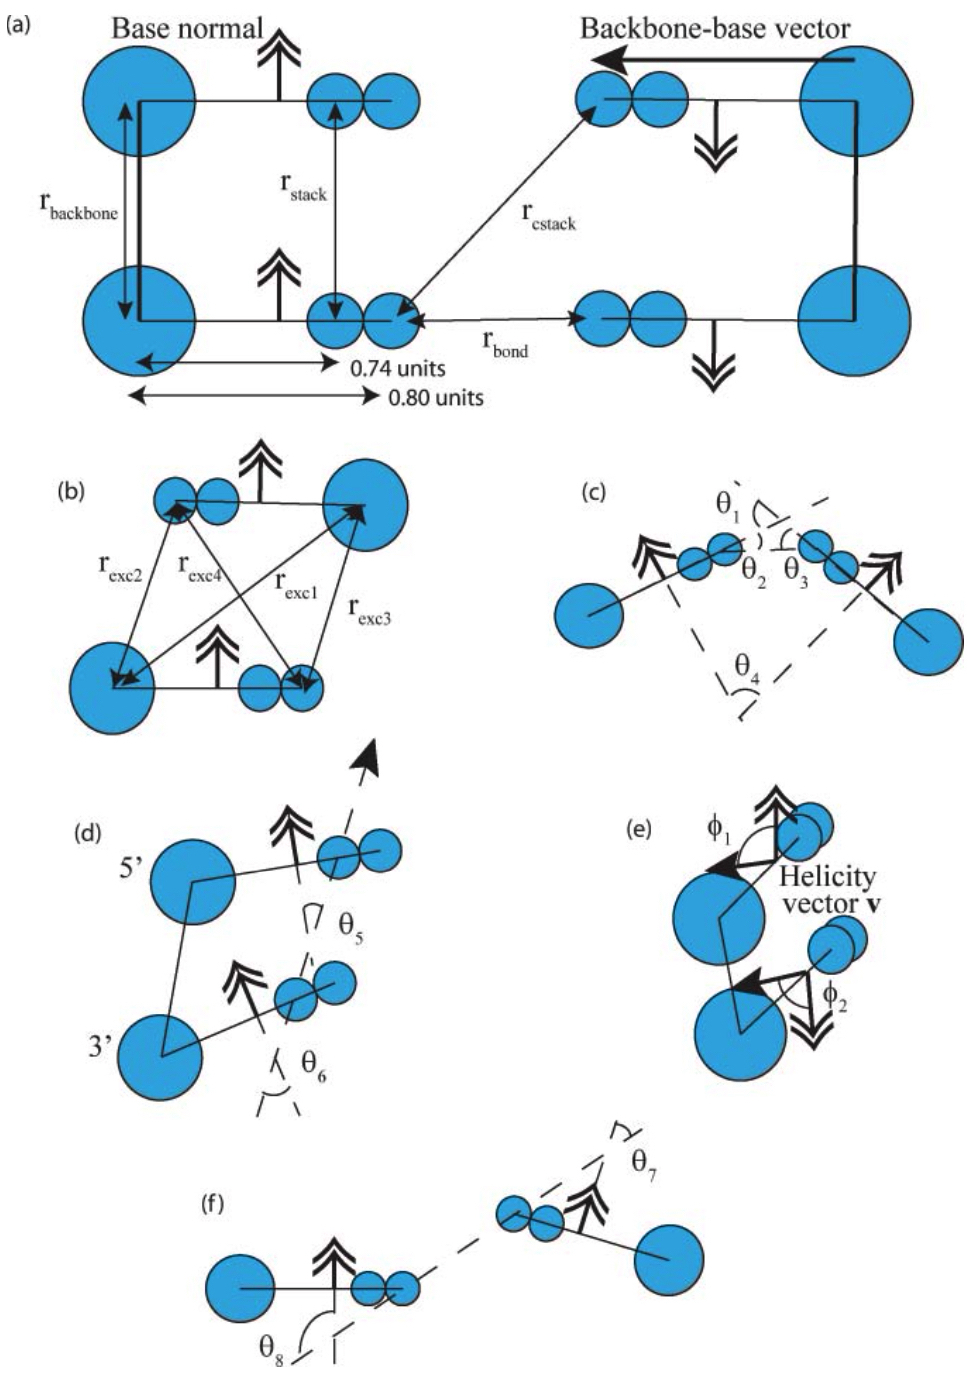
\includegraphics[width=0.9\textwidth]{oxdna.jpg}
\end{center}
\end{column}
\end{columns}

\end{frame}

\begin{frame}
\frametitle{Potential Forms}
Elementary potentials are used, which take distances or angles as arguments.\\[10pt]
\begin{itemize}
\setlength\itemsep{7pt}
\item FENE springs for backbone connectivity\\
$V_{FENE}(r,\epsilon,r^0,\Delta)=-\frac{\epsilon}{2}\ln\left(1-\frac{(r-r^0)^2}{\Delta^2}\right)$
\item Morse potential for stacking and hydrogen-bonding\\
$V_{Morse}(r,\epsilon,r^0,a)=\epsilon(1-\exp(-a(r-r^0)))^2$
\item Harmonic potential for cross-stacking and coaxial stacking\\
$V_{harm}(r,k,r^0)=\frac{k}{2}(r-r^0)^2$
\item Lennard-Jones potential for excluded volume\\
$V_{LJ}(r,\epsilon,\sigma)=4\epsilon\left(\left(\frac{\sigma}{r}\right)^{12} - \left(\frac{\sigma}{r}\right)^6\right)$
\item Quadratic terms for angular modulations\\
$V_{mod}(\theta,a,\theta^0)=1-a(\theta-\theta^0)^2$
\item Quadratic smoothing terms for truncation\\
$V_{smooth}(x,b,x^c)=b(x-x^c)^2$
\item Debye-H\"uckel potential for elextrostatics\\
$V_{DH}(r, \lambda)=\frac{q_{eff}}{4\pi\epsilon_0\epsilon_r} \exp(-r/\lambda)/r$
\end{itemize}

\end{frame}

\begin{frame}
\frametitle{Modulation Factors}
The above potentials are used directly or in angular and radial modulation factors $f_{1,\dots,6}$.
\scriptsize
\begin{flalign*}
  &f_{1}(r) = 
   \begin{cases}
  V_{Morse}(r, \epsilon, r^{0}, a) &\mbox{if } r^{low} < r < r^{high}, \\
  \epsilon V_{smooth}(r, b^{low}, r^{c,low}) &\mbox{if } r^{c, low} < r < r^{low}, \\
  \epsilon V_{smooth}(r, b^{high}, r^{c,high}) &\mbox{if } r^{high} < r < r^{c, high}, \\
  0 &\mbox{otherwise}
  \end{cases}\\
  &f_{2}(r) = 
  \begin{cases}
  V_{harm}(r, k, r^{0})-V_{harm}(r^{c}, k, r^{0}) &\mbox{if } r^{low} < r , r^{high}, \\
  kV_{smooth}(r , b^{low}, r^{c,low}) &\mbox{if } r^{c, low} < r < r^{low}, \\
  kV_{smooth}(r , b^{high}, r^{c,high}) &\mbox{if } r^{high} < r < r^{c, high}, \\
  0 &\mbox{otherwise}
  \end{cases}\\
  &f_{3}(r) = 
  \begin{cases}
  V_{LJ}(r, \epsilon, \sigma) &\mbox{if } r < r^{\star}, \\
  \epsilon V_{smooth}(r, b, r^{c}) &\mbox{if } r^{\star} < r < r^{c}, \\
  0 &\mbox{otherwise}
  \end{cases}\\
  &f_{4}(\theta) = 
  \begin{cases}
  V_{mod}(\theta, a, \theta^{0}) &\mbox{if } \theta^{0} - \Delta\theta^{\star} < \theta < \theta^{0} + \Delta\theta^{\star}, \\
  V_{smooth}(\theta, b, \theta^{0} - \Delta\theta^{c}) &\mbox{if } \theta^{0} - \Delta\theta^{c} < \theta < \theta^{0} - \Delta\theta^{\star}, \\
  V_{smooth}(\theta, b, \theta^{0} + \Delta\theta^{c}) &\mbox{if } \theta^{0} + \Delta\theta^{\star} < \theta < \theta^{0} + \Delta\theta^{c}, \\
  0 &\mbox{otherwise}
  \end{cases}\\
  &f_{5}(x) = 
  \begin{cases}
  1 &\mbox{if } x > 0, \\
  V_{mod}(x,a,0) &\mbox{if } x^{\star} < x < 0, \\
  V_{smooth}(x, b, x^c) &\mbox{if } x^{c} < x< x^{\star}, \\
  0 &\mbox{otherwise}
  \end{cases}\\
  &f_{6}(\theta) = 
  \begin{cases}
  V_{smooth}(\theta, b, \theta^c) &\mbox{if } \theta\ge\theta^{c}, \\
  0 &\mbox{otherwise}
  \end{cases}\\
\end{flalign*}

\end{frame}

\begin{frame}
\frametitle{Interactions}
The oxDNA2 potential consists of 1 bonded and 6 pair interactions.
\vspace*{0.25cm}
\begin{itemize}
\setlength\itemsep{5pt}
\small
\item Backbone connectivity (bonded): $V_{backbone} = V_{FENE}(.)$
\item Excluded volume (pair)\\
$V_{excv} = f_3(r_{back-back}, ..)+f_3(r_{back-base}, ..)+f_3(r_{base-back}, ..)+f_3(r_{base-base}, ..)$
\item Stacking (pair): $V_{stack} = f_1(\cdot)\times f_4(\cdot)\times f_4(\cdot)\times f_4(\cdot)\times f_5(\cdot)\times f_5(\cdot)$
\item Hydrogen-bonding (pair): $V_{HB} = f_1(\cdot)\times f_4(\cdot)\times f_4(\cdot)\times f_4(\cdot)\times f_4(\cdot)\times f_4(\cdot)$
\item Cross-stacking (pair)\\
$V_{x-stack} = f_2(\cdot)\times f_4(\cdot)\times f_4(\cdot)\times f_4(\cdot)\times\Big\{f_4(\cdot)+ f_4(\cdot)\Big\} \times \Big\{f_4(\cdot)+ f_4(\cdot)\Big\} \times\Big\{f_4(\cdot)+ f_4(\cdot)\Big\}$
\item Coaxial stacking (pair)\\
$V_{coaxial-stack} = f_2(\cdot)\times f_4(\cdot)\times \times\Big\{f_4(\cdot)+ f_6(\cdot)\Big\} \times \Big\{f_4(\cdot)+ f_4(\cdot)\Big\} \times\Big\{f_4(\cdot)+ f_4(\cdot)\Big\}$
\item Electrostatic (pair): $V_{elec} = V_{DH}(\cdot)$
\end{itemize}

\vspace*{0.25cm}
The complete potential contains sums over consecutive nucleotides on the same strand and all other pairs.
\begin{flalign*}
V = &\sum_{nearest\ neighbours}(V_{backbone} + V'_{excv} + V_{stack}) \\ 
+ &\sum_{other\ pairs}(V_{elec} + V_{HB} + V_{x-stack} + V_{coaxial-stack} + V_{elec})
\end{flalign*}

\end{frame}


\begin{frame}
\frametitle{Summary}
\vspace*{0.25cm}
\small
\begin{itemize}
\setlength\itemsep{5pt}
\item The oxDNA model uses a \textbf{top-down coarse-graining approach} with rather complex \textbf{bespoke interactions}.
\item The oxDNA potential uses \textbf{one bonded interaction} and \textbf{six pair interactions}. As strands denature, there is no residual memory of other conformations as is often the case with 3+ body interactions.
\item The \textbf{thermodynamic properties} of oxDNA are basically those of the \textbf{SantaLucia nearest-neighbour model}, thought to be an \textbf{exact empirical fit} experiments. 
\item \textbf{Uniquely among coarse-grained  models} at this level of detail, oxDNA is able to describe the \textbf{thermodynamics of duplex formation} and provide an \textbf{accurate average representation} of the structure and mechanics of \textbf{both single-stranded and double stranded DNA and its assemblies}.
\end{itemize}
\vspace*{0.25cm}
\textbf{References}\\[3pt]
[1] T. Ouldridge, A. Louis, and J. Doye, Structural, Mechanical, and Thermodynamic Properties of a Coarse-Grained DNA Model, \textit{J. Chem. Phys.} \textbf{134}, 085101 (2011).\\[3pt]
[2] B. Snodin et al., Introducing Improved Structural Properties and Salt Dependence into a Coarse-Grained Model of DNA, \textit{J. Chem. Phys.}  \textbf{142}, 234901 (2015).

\end{frame}


\section{oxDNA Software}

\begin{frame}
\frametitle{LAMMPS version}


\end{frame}
\section{oxDNA Software}

\begin{frame}
\frametitle{LAMMPS version}


\end{frame}
\section{oxDNA Software}

\begin{frame}
\frametitle{LAMMPS version}


\end{frame}

\begin{frame}
\frametitle{Standalone version}


\end{frame}
\begin{frame}
\frametitle{Standalone version}


\end{frame}
\begin{frame}
\frametitle{Standalone version}


\end{frame}

\section{Practical}

\begin{frame}
\frametitle{Melting}
BlaBlaBlaBlub

\end{frame}

\end{document}
